 % Utilisez la macro de langue appropriée.
 % Noter que toutes les parties du document,
 % à part les articles, doivent être en français.
 % Pour rédiger une thèse en anglais, il faut
 % une permission. Consulter le guide de présentation
 % des mémoires et des thèses pour de l'information
 % plus détaillé et à jour.
%%\francais   %ou
\anglais
\doublespacing
\chapter*{Introduction}

\section{A case for tools and methods}

The way that species interact with one another provides us with a `point of
departure' from which to study or understand biodiversity and the
environment at a range of scales \cite{Jordano2016ChaEco}. This ranges from
understanding how interactions can shape and drive population dynamics,
the maintenance and functioning of ecosystems, as well as long-term
evolutionary dynamics \cite{Landi2018ComSta, Albrecht2018PlaAni}.
Species interactions (and the resulting networks) can be formalised
and viewed under the lens of graph theory \cite{Dale2010GraSpa} - with
species being nodes and interactions being edges. This provides us with
a robust framework built on a mathematical foundation from which to approach
network analysis and quantify various measures of network structure and
behaviour \cite{Delmas2019AnaEco}.

In the process of assembling ecological networks as graphs we are also
`encoding' an `ecological fingerprint' for that community. This raises
the question of how far we can take the idea of `decoding' networks
by leveraging the mathematical framework to better understand the
information that they contain. In particular by leaning on the
mathematical properties (and the ecological information they represent)
to make network predictions, and as a means to provide us with more
information as to how networks may vary over time or spatial scales.

Although the field of network ecology might have a strong conceptual and
theoretical basis from which to work with, we are still at somewhat of a
loss when is comes to our ability to leverage this framework to make any
generalised or macroecological conclusions about the properties of networks
over larger geographic scales (although see \cite{Baiser2019Ecogeographical, Pinheiro2023Latitudinal} who explicitly try and tie networks to classical macroecological theories/laws). This limited understanding can (at least in a large part) be attributed to the sparse global coverage of interaction data \cite{Poisot2021GloKno, Cameron2019UneGlo}, which itself is driven by the immense challenges associated with observing and recording interactions in the field \cite{Bennett2019PotPit, Jordano2016SamNet}. Given the limited feasibility of being able to curate interaction datasets in a way that will result in a global coverage it makes sense to turn to predictive methods as a way to begin filling in the 'gaps' of the global map of interaction data. Although this may seem a daunting task we can lean on the mathematical formalisation and the information that networks contain to make this a possibility, once we have crossed that bridge (\emph{i.e.,} filled the global gaps) we may then find ourselves in a position to be able to ask more global-minded questions \cite{Windsor2023Using, ThuillerNavigating}.

This pipeline from prediction to global questions is shown in \autoref{fig:plan} and is the mainstay of this thesis document \emph{i.e.,} the thesis itself can be thought of as two parts. The first part is addressing the need for predictive tools and discusses as well as develops methods we can use to begin filling in the global map. The second phase of the thesis briefly touches on some new 'tools' we can use when we start to think about large scale questions pertaining to network properties, specifically the question of network complexity (and how the definition thereof matters), as well as detecting boundaries between networks.

\begin{figure}[h]
    \centering
    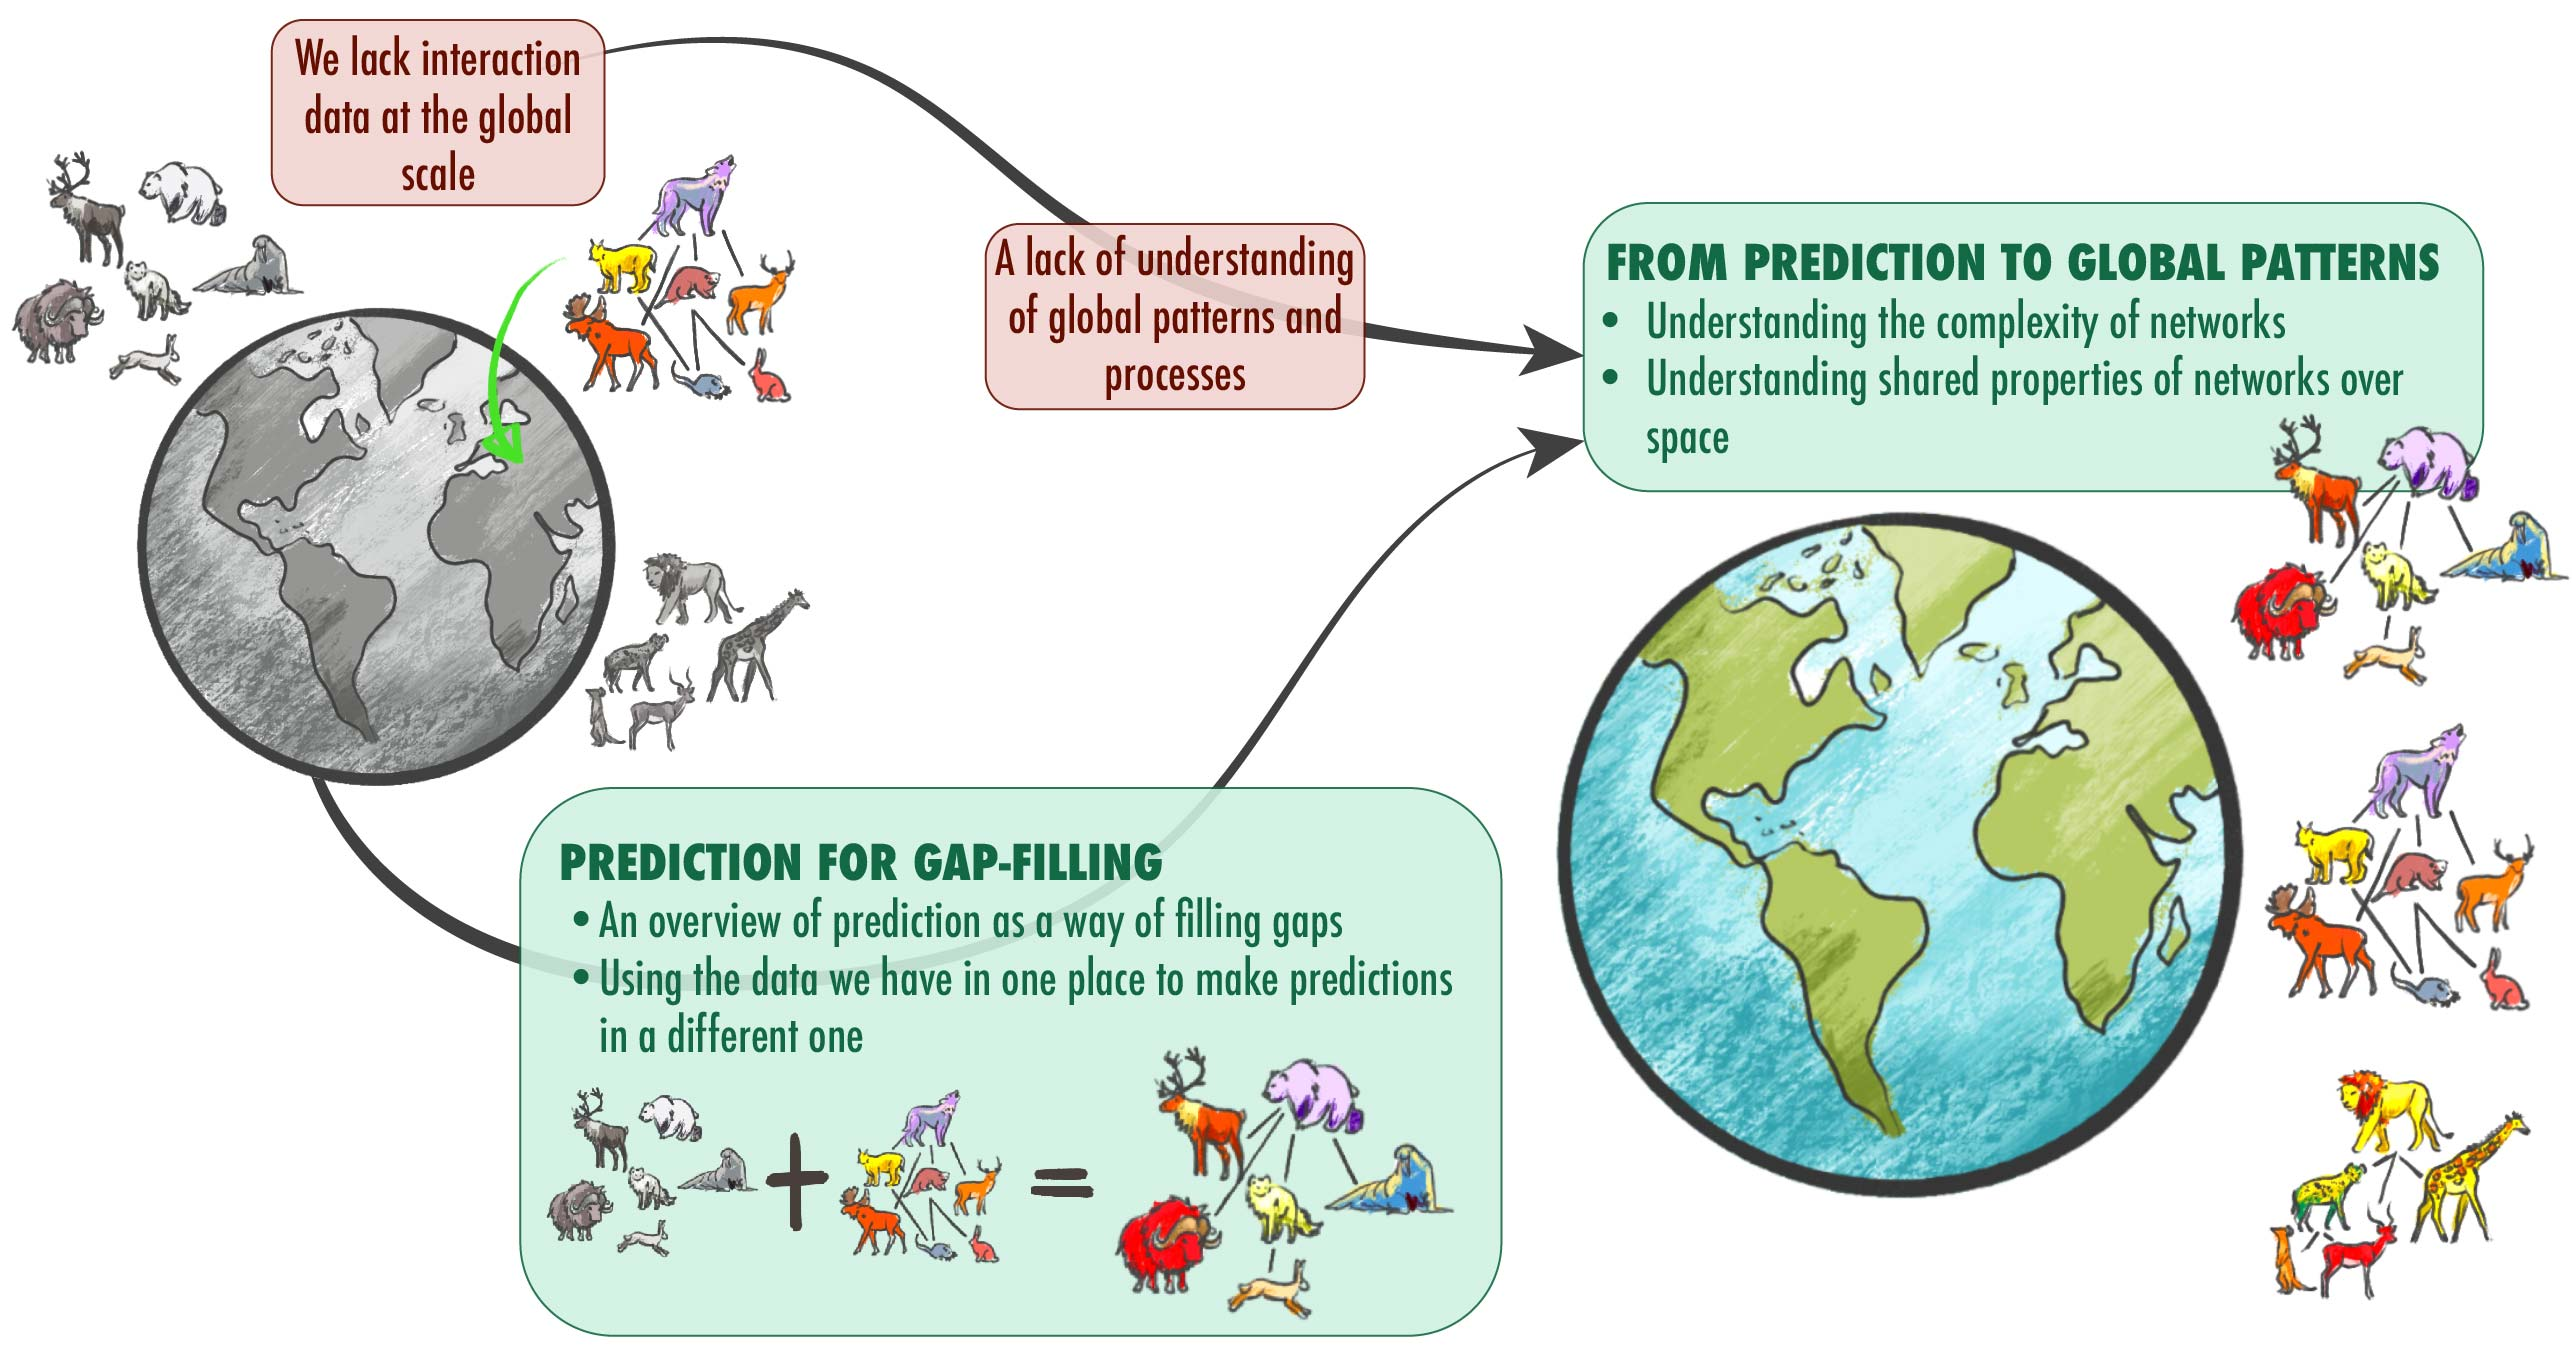
\includegraphics[width=\textwidth]{figures/thesis-flowchart.jpg}
    \caption{One of the biggest factors limiting our ability to ask global questions about ecological networks is the lack of global data. This figure provides a high-level overview of how the development and adoption of predictive methods will equip us to begin asking and answering large-scale questions.}
    \label{fig:plan}
\end{figure}

\subsection{Prediction for gap-filling}

Current methods for network prediction are often conceptualised around and focused on a single facet of species interactions, such phylogenetic matching \cite{Pomeranz2018InfPre, Elmasri2020HieBay}, or functional traits \cite{Bartomeus2016ComFra}. More recently applications of ensemble modelling \cite{Becker2020PreWil} and discussions on the potential of machine learning methods \cite{Desjardins-Proulx2019ArtInt} show promise in addressing methodological constraints to prediction and the growth of open tools and data may mitigate some data constraints in the coming years. However, we still lack a clear path forward or research agenda as to how we can maximise and integrate these resources to allow for ecologically plausible, and accurate, predictions.

The task of trying to predict networks is discussed in chapters \ref{Roadmap} and \ref{Perspectives}, where we map out and discuss some of the methodological considerations we are faced with when trying to approach the task of network prediction. Chapter~\ref{Roadmap} provides a more scoping discussion on these methods, whereas Chapter~\ref{Perspectives} represents a more detailed discussion on the prospect of using graph embedding and transfer learning for network prediction. These specific methods are also the framework presented and used in Chapter~\ref{Foodweb}. This section acts as a 'proof-of-concept' showcasing that the task of network prediction is both attainable and capable of producing ecologically plausible networks.

\subsection{From prediction to global patterns}

Although prediction is a powerful tool in the immediate/local sense 
(\emph{e.g.,} it can allow local land managers/custodians to have a 
first approximation of how species may be interacting in that given area it is of course also a feasible way to fill in the global interaction network map. A 'filled map' will put us in the position to develop a more mechanistic, global-scaled, understanding of networks. Specifically, we need tools that will allow us to use the \emph{correct} methodology when comparing networks form different regions (\autoref{SVD}) and we can begin to leverage those data to understand the spatial structure of networks (\autoref{SpatialBoundaries}). Chapter~\ref{SVD}, which presents a different, more information theory approach to defining complexity using the singular value vector component of an SVD \cite{Shannon1948MatThe}, and the final chapter of this thesis (\autoref{SpatialBoundaries}) is a \texttt{Julia} package that allows users to implement the Wombling algorithm (an edge detection mechanism; \cite{Womble1951DifSys}).

Ecological networks have always been deemed to be ``complex'', and an interest in the notion of complexity has (in part) been tied to network stability \cite{Landi2018ComSta}. However the relationship between complexity and stability remains inconsistent when rigorously tested on empirical datasets \cite{Jacquet2016NoCom}, and although ecological networks may be complex, the ways that we currently define complexity do not translate into predictions about their stability. Traditionally network ecology readily assumes that because this system has more components (\emph{e.g.,} links) it means that the system itself is complex. In \autoref{SVD} we challenge the more traditional structural (`behavioural') measures of  complexity and present SVD entropy as an alternative ('physical') measure of complexity.

Being able to subdivide networks into patches within a landscape will help us to better understand the boundaries of (and between) networks as well as how these may relate to species or community changes and boundaries - such as when transitioning across habitat `boundaries' \cite{Hackett2019ResOur}. Wombling has been discussed as a useful tool for spatial analyses in ecology \cite{Fortin2005SpaAna} and has been used to detect transitions across a landscape \cite{Philibert2008SpaStr}, changes in biological variables in communities \cite{Barbujani1989DetReg} and to analyse the spread of invasive species \cite{Fitzpatrick2010EcoBou}.

\subsection{Objectives}\label{objectives-and-hypotheses}

Being able to understand, quantify, and work with ecological networks is
important from a conservation and land management perspective as this
will have cascading implications with regards to ecosystem functioning
and stability. Yet we are severely hindered by a lack of high-quality,
usable data as well as an appropriate set of tools that can be used to
contextualise and understand ecological networks. There is a need for
tools that can help us construct networks for where there are no data
\emph{i.e.,} make predictions as well as developing tools (or ideas) that
can be used to help further our mechanistic understanding of networks once
we are at a point where we have the large scale data to do so. My work will
help address these two issues in the context of developing tools that will
either directly enable us to make predictions (Chapters~\ref{Roadmap},
\ref{Perspectives}, and \ref{Foodweb}), or present methods that are aligned
with global (large-scale) questions that will allow us to compare networks
(Chapter~\ref{SVD}) or attempt to delineate them 
(Chapter~\ref{SpatialBoundaries}).

\section{Overview of key methodological approaches}

\subsection{Transfer learning for network prediction}\label{transfer-learning-for-network-prediction}

Transfer learning is a machine learning methodology that uses the 
knowledge gained when solving a known problem and
applying it to solve a (related) problem by transferring the knowledge
across a shared medium (space) \cite{Torrey2010TraLea, Pan2010SurTra}.
The concept of transfer learning is an approach that is particularly well suited for the problem of network
prediction as it allows us to lean on the data that are available to 
enable us to make \emph{de novo} interaction network predictions. This could be as simple as pinpointing missing interactions in the existing data 
(\emph{e.g.,} pairwise learning has been used to predict plant-pollinator
interactions \cite{Stock2021PaiLea}) as well as a way to predict
novel interactions (\emph{i.e.,} fill in those global gaps) in a different location. This, in a sense, allows us to bring knowledge with us from an area for which we \emph{have} data to an area where it is \emph{lacking}. In the case of predicting species interactions, transfer learning is useful because interactions are phylogenetically conserved and thus phylogenetic relatedness can be used to predict interactions \cite{Davies2021EcoRed, Elmasri2020HieBay, Gomez2010EcoInt}. Chapter~\ref{Foodweb} presents a transfer learning framework and uses the task of constructing a Canadian metaweb (a list of all possible interactions for a species pool) using the European metaweb assembled by \cite{Maiorano2020TetSpe} as a proof-of-concept. Below is a high-level summary of that framework, and a more detailed description of the workflow can be found \href{https://osf.io/2zwqm/}{\texttt{here}}.

\subsubsection{Learning using graph embedding}\label{learning~using~embedding}

Before one can transfer any knowledge we must first learn something about the system using known interaction network. Since ecological networks can be represented by their adjacency matrices we can turn to graph theory to help us find a way to learn something about the known interaction network. Graph embedding is a low dimensional representation of the graph (interaction network) but, importantly, still preserves its topology \cite{Yan2005Graph}. This process essentially allows us to learn something about where species (nodes) are situated within the network - which (in an abstract way) informs us of the role a species plays in the community (\emph{e.g.,} the `predator-ness' or `prey-ness' of a species). There are multiple embedding approaches discussed in Chapter~\ref{Perspectives}, but in the context of the framework developed in Chapter~\ref{Foodweb} we will focus on the use of SVD as an embedding technique. SVD presents an appropriate embedding of ecological networks, having been shown to both capture their complex, emerging properties \cite{Strydom2021SvdEnt} and allow for the highly accurate prediction of the interactions within a single network \cite{Poisot2021ImpMam}.

\subsubsection{Graph embedding using SVD}

Singular Value Decomposition \cite{Forsythe1967ComSol, Golub1971SinVal} 
is the factorisation of an adjacency matrix \(\mathbf{A}\) (where
\(\mathbf{A}_{m,n} \in\mathbb{B}\)) into the form:

\[ \mathbf{U}\cdot\mathbf{\Sigma}\cdot\mathbf{V}^T \]

Where \(\mathbf{U}\) is an \(m \times m\) orthogonal matrix and
\(\mathbf{V}\) an \(n \times n\) orthogonal matrix. The columns in these
matrices are, respectively, the left- and right-singular vectors of
\(\mathbf{A}\). \(\mathbf{\Sigma}\) is a diagonal matrix that contains
only non-negative \(\sigma\) values.
 
An SVD can be truncated so as to remove additional noise in the dataset by
omitting non-zero and/or smaller \(\sigma\) values from
\(\mathbf{\Sigma}\) using the rank of the matrix. Under a t-SVD
\(\mathbf{A}_{m,n}\) is decomposed so that \(\mathbf{\Sigma}\) is a
square \(r \times r\) diagonal matrix (whith \(1 \le r \le r_{full}\)
where \(r_{full}\) is the full rank of \(\mathbf{A}\) and \(r\) the rank
at which we truncate the matrix). Additionally, \(\mathbf{U}_{t}\) is now a
\(m \times r\) semi unitary matrix and \(\mathbf{V}'_{t}\) an \(n \times r\)
semi-unitary matrix.

In the context of 'learning using embedding' the learned information is captured using an SVD, however for the task of network prediction we modified the products of the SVD so that they could be used for an RDPG. An RDPG  estimates the probability of observing interactions between nodes (species) as a function of the latent variables of the nodes. An RDPG allows us to turn an SVD (which consists of three matrices) into two matrices that can be multiplied to provide an approximation of the network. The latent variables used for the RDPG, called the left and right subspaces are thus constructed from an SVD and are defined as $\mathscr{L} = \mathbf{U}\sqrt{\mathbf{\Sigma}}$, and $\mathscr{R} = \sqrt{\mathbf{\Sigma}}\mathbf{V}'$ -- using the full rank of $\mathbf{A}, \mathscr{L}\mathscr{R} = \mathbf{A}$, and using any smaller rank results in $\mathscr{L}\mathscr{R} \approx \mathbf{A}$. These subspaces are ecologically informative and tell us about the 'generality' (think predator capacity, \emph{sensu} \cite{Schoener1989FooWeb}) and  'vulnerability' (think capacity to be prey, \emph{sensu} \cite{Schoener1989FooWeb}) of the species in the European network. This in essence provides us with an idea of where a species is likely to occur within a network/the space it occupies in the network.

\subsubsection{Transferring and inferring using phylogenetic relatedness}

In order to transfer the knowledge (the generality and vulnerability values) from a known network to the destination species pool (\emph{i.e.,} a community for which we have no interaction data), we performed ancestral character estimation using a Brownian motion model and the Upham \cite{Upham2019InfMam} mammalian phylogeny. This uses the estimated feature vectors (left and right subspaces) for the species from the known network to create a state reconstruction for all species and allows us to impute the missing generality and vulnerability values for the destination species pool that are not already in the known network. Essentially this allows us to infer where in the two subspaces the destination species are located.

\subsubsection{Novel Prediction using RDPG}

As we now essentially have the left and right subspaces for the destination species pool we can directly multiply these to yield the metaweb, specifically using an RDPG. Because of how the phylogenetic reconstruction was implemented the left and right subspaces have an associated uncertainty, therefore, we can assemble a \emph{probabilistic} metaweb, \emph{sensu} \cite{Poisot2016StrPro}, \emph{i.e.,} in which every interaction is represented as a single, independent, Bernoulli event of probability \(p\).

\subsection{SVD entropy: a measure of network
complexity}\label{svd-entropy-a-measure-of-network-complexity}

We can also use SVD as a way to define the complexity of a network. Two potential candidate measures of complexity can be derived based on the `physical structure' of (\emph{i.e.,} information within) a network. The first measure is the rank of the matrix. The rank of $\mathbf{A}$ (noted as $r = \text{rk}(\mathbf{A})$) is the dimension of the vector space spanned by the matrix and corresponds to the number of linearly independent rows or columns, which works as an estimate of its `external complexity', since it describes the dimensionality of the vector space of the matrix. Looking at this from an ecological standpoint, we can think of the this as quantifying the number of unique `strategies' within a network.

The second measure is to calculate the entropy of the matrix obtained through SVD by using the singular values \cite{Shannon1948MatThe}. This so-called SVD entropy measures the extent to which each rank encodes an equal amount of information (as the singular values capture the importance of each rank to reconstruct the original matrix) this approach therefore serves as a measure of `internal complexity'.

Intuitively, the singular value $i$ ($\sigma_i$) measures how much of the dataset is (proportionally) explained by each vector - therefore, one can measure the entropy of \(\mathbf{\sigma}\) following \cite{Shannon1948MatThe}. High values of SVD entropy reflects that all vectors are equally important, \emph{i.e.,} that the structure of the ecological network cannot be efficiently compressed, and therefore indicates a high complexity \cite{Gu2016HowLon}. Because networks have different dimensions, we can use Pielou's evenness \cite{Pielou1975EcoDiv} to ensure that values are lower than unity, and quantify SVD entropy, using $s_i = \sigma_i/\text{sum}(\sigma)$ as:

$$J = -\frac{1}{\ln(k)}\sum_{i=1}^k s_i\cdot\ln(s_i)$$

Where \(k = \text{rk}(\mathbf{A})\) \emph{i.e.,} the rank of the matrix, which is equal to the number of non-zero entries in \(\mathbf{\Sigma}\) as per the Eckart-Young-Mirsky theorem \cite{Eckart1936AppOne, Golub1987GenEck}. 

\subsection{Spatial wombling for edge detection}

Spatial wombling (an edge detection algorithm; \cite{Womble1951DifSys}). Chapter~\ref{SpatialBoundaries} presents a \texttt{Julia} package that implements both the lattice and triangulation wombling algorithms. Broadly, wombling interpolates between a given set of points but in addition to looking at the deference between said points it also looks at the direction (slope) of the difference between points. First we can calculat the rate of change \(m\) which is calculated as:

$$m = \sqrt{\frac{\partial f(x,y)}{\partial x}^2 + \frac{\partial
f(x,y)}{\partial y}^2}$$

This can be used to find the zones of rapid change across the landscape and identify potential candidate boundaries (which would be where change is occurring most rapidly). It is also possible to calculate the direction (\(\theta\)) for each rate of change. This is calculated as:

$$\theta = \arctan \left( \frac{\partial f(x,y)}{\partial y} \bigg/ \frac{\partial f(x,y)}{\partial x} \right) + \Delta$$

$$\text{where} \quad \Delta =
\left\{ \begin{array}{ccc}
    0 \degree & \text{if} & \frac{\partial f(x,y)}{\partial x} \geq 0 \\
    180 \degree & \text{if} & \frac{\partial f(x,y)}{\partial x} < 0 \\
\end{array} \right\}$$

Both $m$ and $\theta$ are an approximation on the `topology' of a certain metric ($z$, \emph{e.g.,} number of species) between a collection of points in a landscape. Similarity between the $z$ values indicates a uniformity between those points and thus a low rate of change whereas a high degree of difference between points is indicative of rapid change \emph{i.e.,} a boundary as we transition from one zone to the next.

\subsubsection{Lattice wombling}

For a lattice of points where one will have sampling locations arranged
the 'topology' \emph{i.e.} function of the landscape as determined by $z$ ($f(x,y)$) can be defined as:

$$f(x,y) = z_{1}(1-x)(1-y) + z_{2}x(1-y) + z_{3}x y + z_{4}(1-x)y$$

\subsubsection{Triangulation wombling}

When working with points that are irregularly distributed across the landscape it is possible to use triangulation wombling \cite{Fortin1995DelEco}. The three nearest neighbours can be determined using a Delaunay triangulation algorithm \cite{Delaunay1934SphVid} and $f(x,y)$ can be defined as:

$$f(x,y) = ax + by + c$$

where:

$$ \left[ \begin{array}{ccc} a & b & c \end{array} \right] = 
\left[ {\begin{array}{ccc}
   x_{1} & y_{1} & 1\\
   x_{2} & y_{2} & 1\\
   x_{3} & y_{3} & 1\\
  \end{array} } \right]^{-1}\cdot
  \left[
  \begin{array}{ccc} z_{1} & z_{2} & z_{3} \end{array} \right]$$

and the position of the centroid between points is calculated as follows:

$$ \Big( \frac{x_{1} + x_{2} + x_{3}}{3} \Big), \Big( \frac{y_{1} + y_{2} +
y_{3}}{3} \Big) $$

\subsubsection{Boundary detection}

Detecting boundaries \emph{i.e.,} areas where the angle of the landscape
transitions sharply is surprisingly simple. After having calculated the
rate of change (\(m\)) for the geographical area it is possible to use
these values to identify and assign potential boundaries
\cite{Fortin2005SpaAna, Oden1993CatWom, Fortin1995DelEco}. Following the
approach outlined in \cite{Fortin2005SpaAna} a threshold value (or
percentile class) can be set and will determine what proportion of cells
will be retained as potential boundaries.

\section{Chapter summaries}

\subsection{Chapter 1: A roadmap for predicting ecological networks}

Chapter~\ref{Roadmap} maps out a series of questions and considerations with regards to approaching the challenge of predicting species interactions across space and time. This chapter represents a scoping overview of the 'gap-filling' portion of this thesis and strongly focuses on the idea of networks as predictable objects. \autoref{predicting-species-interaction-networks-across-space-challenges-and-opportunities} starts by outlining the challenges that might limit our ability to predict networks (which is primarily due to a limitation in data) but also looks into the opportunities we have to try and circumvent or overcome these limitations. Overall this section highlights the fact that one of the most limiting factors for prediction (a lack of data) is also the reason we need predictive tools (to overcome the lack of data), and that we are (methodologically and computationally) in a place where we can start to make feasible predictions, particularly if we think about combining different data sources.

Sections~\ref{a-case-study-deep-learning-of-spatially-sparse-host-parasite-interactions} does exactly this by providing a proof-of-concept showcasing the use of co-occurrence and known interactions to predict novel interactions. This is done using the Hadfield dataset \cite{Hadfield2014TalTwo}, which describes 51 host-parasite networks sampled across space. Essentially this showcases how we can extract features for each species based on co-occurrence, use said features to train an artificial neural network to predict interactions, and apply this classifier to the original features to predict potential interactions across the entire species pool. This framework essentially allows us to 'correct' any false negatives (interactions recorded as missing but are actually plausible) within the existing data. This is particularly meaningful as interactions intrinsically vary across space and time, and given the number of species that compose ecological communities, it can be tough to distinguish between a true negative (where two species never interact) from a false negative (where two species have not been observed interacting even though they actually do).

The final part of this manuscript (\autoref{a-primer-on-predicting-ecological-networks}) aims to provide a practical overview of different components to think about and take into consideration when wanting to predict networks. This body of work is intended to be something that can be taken and used as a brief primer, and as such focuses on discussing some fundamental ideas and concepts. This includes breaking down aspects of the modelling process, aspects of species interaction networks (and the interactions within them), and predicting networks over space and time. As a whole, this chapter really serves to sketch out the 'nuts and bolts' of wanting to take on the task of network prediction and serve as a useful roadmap for those wishing to find a more practical and attainable approach to addressing the global interaction data shortage.

\subsection{Chapter 2: Graph embedding for network prediction}

This chapter should be viewed as a prospective companion piece to the more ''tangible'' methods presented in \autoref{Foodweb}, and is strongly rooted in the realm of thinking about network prediction. This chapter is still related to the idea of transfer learning for network prediction, however it focuses more on the expanding how we think about (and can use) a metaweb, as well as potential (alternative) graph embedding methodologies. This chapter thus pushes forward the 'we need gap-filling methods' agenda of this thesis and helps in providing a larger discussion as to the alternative ways we can modify and approach the transfer learning framework from \autoref{Foodweb}.

Section~\ref{a-metaweb-is-an-inherently-probabilistic-object} provides a discussion on how we can push the original definition of a metaweb developed by \cite{Dunne2006NetStr} in a new 'prediction friendly' direction. As the term 'metaweb' has been used multiple times it is perhaps useful to define it with regards to its original function -- to act as an inventory of all possible interactions for a given community. This means that as a concept a metaweb is a realistic, and attainable object to try and predict, however, it is beneficial to move away from thinking of the interactions in a metaweb as binary and rather define the interactions as Bernoulli events. Fundamentally this will allow us greater flexibility in how we weight rare interactions, provide a more nuanced overview of how the community is actually interacting, or factor in a sense of 'uncertainty' into our predictions.

\autoref{graph-embedding-offers-promises-for-the-inference-of-potential-interactions} provides a more detailed overview and discussion of how graph embedding works and why it is a useful way to approach network prediction. This section also includes examples of different graph embedding techniques, and (where possible) their applications to network ecology. The fundamental argument in favour of using network embedding for network prediction is that it is capturing elements of the \emph{structure} of a network (as opposed to pairwise learning of species $a$ eats $b$) and thus provides a more powerful abstraction of a network that can be used for predicting networks for other, non-related, communities. There is also an illustration of the embedding process, which is discussed in \autoref{an-illustration-of-metaweb-embedding} and acts as a way to showcase how the embedding process captures ecological processes. A more in-depth tutorial/breakdown of the analysis can be accessed through \autoref{supp:perspectives}.

The final section (\autoref{identifying-the-properties-of-the-network-to-embed}) is more focused on the limitations and scope of network embedding and prediction. There is a particular focus on the limitations of taxonomic overlap and the need for 'just the right amount' of species to be shared between known and target communities. There is of course also the challenge of political scale and how the construction of metawebs are at regional scales that may not be ecologically relevant (but are relevant for policy making). Although we are not able to confidently provide a solution for this problem (as we do not even know what an 'ecologically relevant scale' is) it is still important to think about and grapple with these topics.

\subsection{Chapter 3: Prediction in action: The Canadian Metaweb}

Building on the ideas in \autoref{Roadmap}, work on the use of 
transfer learning for predicting \emph{de novo} interactions
\cite{Runghen2021ExpNod}, and the applicability of phylogenetic
reconstruction within the context of ecological networks \emph{e.g.,}
\cite{Braga2021PhyRec}, we set out to create a probabilistic metaweb for
terrestrial Canadian mammals in \autoref{Foodweb}. Despite their importance in many ecological processes, collecting data and information on ecological interactions is an exceedingly challenging task. For this reason, large parts of the world have a data deficit when it comes to species interactions and how the resulting networks are structured. A key premise of this chapter is the idea of being able to take the information that we do have and bring it with us to predict networks in an area where we have no information. This is fundamentally a chance to 'put our money where our mouth is' and provide a \emph{tangible} way to approach (and round out) the gap-filling portion of this thesis. Specifically, this framework allows us to ‘learn’ the information (latent traits) of species from a known interaction network (in this case, the European metaweb) and infer the latent traits of another species pool for which we have no \emph{a priori} interaction data (in this case Canadian species) based on their phylogenetic relatedness to species from the known network (see section~\ref{transfer-learning-for-network-prediction} for a more detailed summary of the methodology). 

Using the prediction of the Canadian metaweb as a way to test the methodology presented in this chapter is useful as we have existing datasets with which to test the validity of our predictions. What is perhaps most exciting about this chapter is that despite sharing about only 4\% of species between Canada and Europe we were able to construct a metaweb that correctly predicted about 91\% of the species interactions in Canada. It should also be noted that when comparing  the European and Canadian metawebs we see a difference in their structures (\autoref{rdpg-reconstructed-networks-have-diverse-structures}), implying that the embedding process is not 'copy pasting' the European network and filling in Canadian species but rather capturing an ecological process.

In addition to testing the validity of the predicted interactions within the Canadian metaweb we also did some additional tests using just the European metaweb. In this instance interactions within the European network were modified (either removed or new interactions were added) and the modified network was used to predict a 'new' European network. This allowed us to compare how well the model could recover the original network despite being 'given' erroneous information. Overall the model is robust to both the addition as well as removal of interactions, although the removal of interactions does have a more negative effect on the ability of the model to recover interactions (\autoref{rdpg-yields-an-accurate-classifier})

Overall it appears that the transfer learning framework presented in this chapter is quite robust and has potential applicability in a variety of settings (\emph{e.g.,} generating metawebs that can be used as `informative priors' from which more localised/spatially explicit networks can be constructed \cite{Cirtwill2019QuaFra}), can be given to a local expert for more refined validation, and overall presents a potential mechanism to begin filling in the global gaps.

\subsection{Chapter 4: SVD entropy: a measure of network complexity}

In \autoref{SVD} we present SVD entropy as a starting point to
unifying (and standardising) how we define the complexity of ecological
networks. In the perspective of 'global questions about patterns' this of course presents a way in which we can ask a simple question - do different networks (in the case of this chapter different bipartite networks) have differences in their complexity. What makes SVD entropy a compelling metric for quantifying complexity (when comparing to the more 'standard', structural measures such as nestedness, connectance, and spectral radius) is that it focuses more on the 'physical' complexity of the network as opposed to the complexity of the behaviour of the system. This is because the structural measures of complexity are capturing an emerging property of the network, whereas SVD entropy captures the information contained in the the network (one can think of this as the 'compressibility' of the network, more complex networks are harder to compress).

The primary take away from this chapter is that (at least bipartite networks) are exceptionally complex. In \autoref{most-ecological-networks-are-close-to-full-rank} we can see that networks have a relative rank deficiency of zero (\emph{i.e.,} they have a maximal 'external complexity') and all networks have an SVD entropy value greater than 0.80, \emph{i.e.,} near maximal 'internal complexity' (for context the way that SVD entropy is calculated means that values are constrained between zero and one). In \autoref{most-elements-of-network-structure-capture-network-complexity} we also looked at the corresponding connectance, nestedness, and spectral radius of these networks . Although there is a correlation between the calculated entropy and these other metrics the story that is told by the different metrics is different. Namely, for the structural metrics the 'complexity' spans the entire potential range of of values, and there is the potential for 'misinterpreting' what could be considered complex. For example networks that have a maximal nestedness have the lowest SVD entropy (\emph{i.e.,} the lowest physical complexity), this is not necessarily the most intuitive way to interpret a maximal nestedness. This 'breakdown' of what complexity means is also echoed in \autoref{complex-networks-are-not-more-robust-to-extinction}, here we simulated extinctions to get a measure of network resilience (since a common adage is that complexity begets stability), however we do not see a strong relationship between SVD entropy and resilience. This again highlights that 'structural' and 'physical' complexity metrics are capturing different facets of a network, and although it is not to say that SVD entropy is a 'better' way to measure the complexity of a network it does highlight that we need to be mindful of how we are defining 'complexity' and particularly how that might impact on how we interpret results based on the complexity of networks.

An additional interesting result discussed in \autoref{larger-networks-are-less-complex-than-they-could-be} is that although the complexity of ecological networks is indeed \emph{immense} they are still not reaching their \emph{maximum} potential complexity, which implies that \emph{something} might be constraining network complexity. This result is echoed in \autoref{connectance-constrains-complexity-but-also-rank-deficiency}, which looks at the relationship between network size, connectance and complexity. Results point to the potential constraint of network size on complexity. One possible explanation is that networks at the early assembly stages tend to be severely constrained \cite{Barbier2018GenAss, Saravia2018EcoNet} due to conditions needed for the persistence of multiple species. As networks grow larger, these constraints may ``relax'', leading to networks with more redundancy, and therefore a lower complexity.

\subsection{Chapter 5: SpatialBoundaries.jl: a software for boundary detection}

In this chapter we present a \texttt{Julia} package \texttt{SpatialBoundaries.jl}, (the documentation is available \href{https://poisotlab.github.io/SpatialBoundaries.jl/dev/}{here}) that has the functionality to implement the spatial wombling algorithm across both a uniform landscape \emph{i.e.,} lattice wombling as well as irregular/random landscapes \emph{i.e.,} triangulation wombling. These two methods still calculate the rate of change (\(m\)) and directionality (\(\theta\)) in the same manner but differ in how the aggregate and quantify the surface for a set of points \cite{Fortin2005SpaAna}. These two algorithms provide functionality for most use cases when data are quantitative. \texttt{SpatialBoundaries.jl} has also been developed so as to integrate with other packages such as \texttt{SimpleSDMLayers.jl}.

Overall this chapter is 'simple' in its content (a software package that can implement the spatial wombling algorithm) however it has been developed with the forward-scoping idea of being used within the context of thinking about boundaries between networks (or if they are even present) and thus aligns well with the idea of developing tools for understanding global/large scale network patterns. Some ideas for implementing this package are presented in \autoref{supp:boundaries}, and primarily rest on the idea of using a combination of a metacommunity model and simulated landscapes to see if networks, species, and environmental boundaries show a high degree of fidelity or not. The work presented in \autoref{supp:boundaries} should be treated as a speculative outline of what we can do with the \texttt{SpatialBoundaries.jl} in the context of network analysis and could be viewed as an rough first draft on trying to understand 'where networks stop?', which echoes one of the challenges discussed in \autoref{Perspectives}, particularly in \autoref{identifying-the-scope-of-the-prediction-to-perform}.

\section{Conclusion}\label{conclusion}

As a whole this thesis should be viewed as a computational toolbox for
network ecology that addresses both the issue of data scarcity through
the use of predictive tools (addressing the `Eltonian shortfall' highlighted by \cite{Hortal2015SevSho}) as well as presenting methods/ideas geared towards thinking about networks at global scales. This means that we would \emph{i}) have `tangible' networks from which we can begin to work with in various contexts or situations and \emph{ii}) have new methods/tools to begin asking questions about networks at a global scale. In other words adding more building blocks from which we can begin to take network ecology to the next level, \emph{i.e.,} bridging the gap from 'local-level network understanding' to 'tools for global network analysis'.

\bibliographystyle{plain}
\sectionbibliography{ref_Intro.bib}

\endinput
%%
%% End of file `introduction.tex'.
